\chapter{Arhitektura i dizajn sustava}
		
		%\textbf{\textit{dio 1. revizije}}\\

		%\textit{ Potrebno je opisati stil arhitekture te identificirati: podsustave, preslikavanje na radnu platformu, spremišta podataka, mrežne protokole, globalni upravljački tok i sklopovsko-programske zahtjeve. Po točkama razraditi i popratiti odgovarajućim skicama:}
	%\begin{itemize}
		%\item 	\textit{izbor arhitekture temeljem principa oblikovanja pokazanih na predavanjima (objasniti zašto ste baš odabrali takvu arhitekturu)}
		%\item 	\textit{organizaciju sustava s najviše razine apstrakcije (npr. klijent-poslužitelj, baza podataka, datotečni sustav, grafičko sučelje)}
		%\item 	\textit{organizaciju aplikacije (npr. slojevi frontend i backend, MVC arhitektura) }		
	%\end{itemize}
				
		Arhitektura naše aplikacije na najvišoj razni apstrakcije odgovara troslojnoj klijent-poslužitelj arhitekturi sa sljedećim slojevima:
		\begin{itemize}
			\item Prezentacijski sloj (Frontend)
			\item Sloj poslovne logike (Backend)
			\item Podatkovni sloj (Baza podataka)
		\end{itemize}

		\begin{figure}[H]
			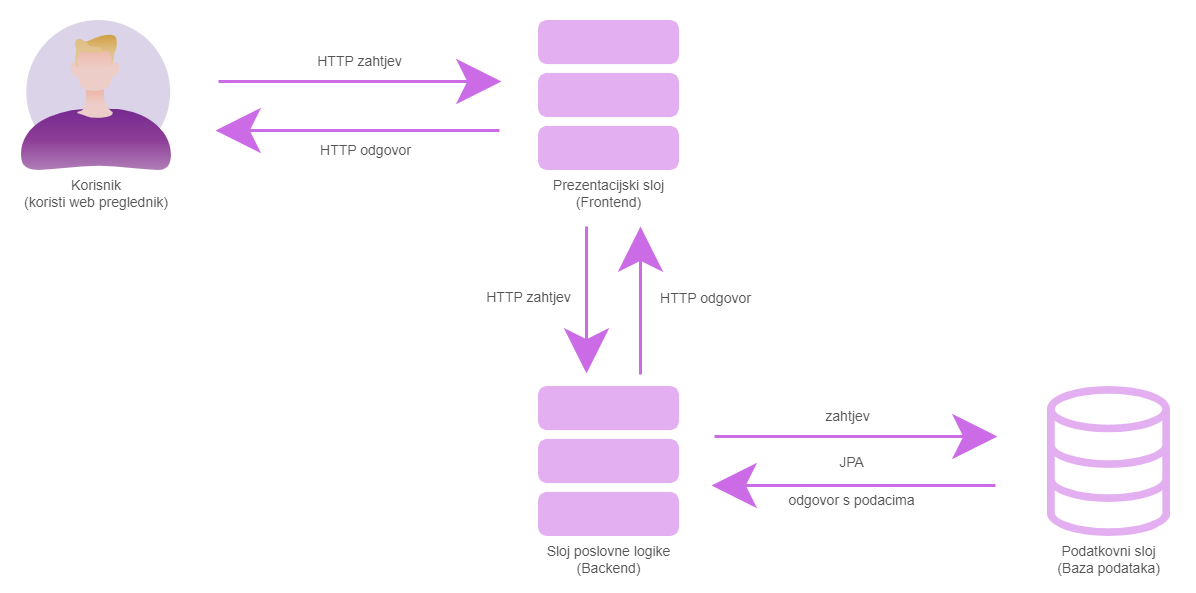
\includegraphics[width=\textwidth,height=0.4\textheight]{slike/Arhitektura.png}
			\centering
			\caption{Arhitektura sustava}
			\label{fig:Arhitektura}
		\end{figure}

		\eject

		Općenito govoreći, prezentacijski sloj tj. frontend zadužen je za prikaz stranice korisniku i omogućavanje rada s istom. S druge strane, sloj poslovne logike tj. backend zadužena je za razne izračune i interakciju s bazom. U ovom pogledu, sloj poslovne logike služi kao spona između prezentacijskog sloja i podatkovnog sloja koja pritom obavlja sve akcije neprikladne za izvođenje na klijentovom računalu - u pitanju je "tanki" klijent.\\[2pt]

		Korisnik koristeći web preglednik pristupa našoj aplikaciji slanjem HTTP zahtjeva prezentacijskom sloju. Prezentacijski sloj u odgovoru šalje sve potrebne podatke za prikaz korisničkog sučelja - naše stranice.
		Kada korisniku treba poslužiti neki sadržaj koji nije pohranjen na prezentacijskom sloju (npr. aktivne donacije, podatci o korisniku i oglasima), prezentacijski sloj sloju poslovne logike šalje HTTP zahtjev - npr. GET zahtjev s ciljem dohvata podataka o djeci korisnika.
		Komunikacija između prezentacijskog sloja i sloja poslovne logike odvija se po REST načelima.\\[2pt]

		Sloj poslovne logike potreban je za kompliciranije izračune, dohvat i izmjenu podataka te odgovaranje na zahtjeve pristigle od strane prezentacijskog sloja.
		Podatkovni sloj tj. baza podataka služi za pohranu svih potrebnih podataka (npr. podataka o registriranim korisnicima, oglasima i predmetima). Pri radu naše aplikacije, s bazom podataka komunicira isključivo sloj poslovne logike tj. backend - ako prezentacijskom sloju trebaju određeni podaci, poslat će zahtjev sloju poslovne logike te u idealnom slučaju u odgovoru dobiti tražene podatke.\\[2pt]

		Prezentacijski sloj tj. frontend izrađen je koristeći programski jezik Javascript zajedno s "markup" jezikom HTML, CSS-om i radnim okvirom React.
		Sloj poslovne logike tj. backend izrađen je koristeći programski jezik Java zajedno s radnim okvirom Java Spring Boot. Za komunikaciju s bazom korišten je JPA - Java Persistence API.
		Shema baze podataka izrađena je koristeći alat ERDplus, a sama baza podataka izrađena je koristeći sustav za upravljanje bazama PostgreSQL.

		\eject
		\section{Baza podataka}
			
		Za naš zadatak odabrali smo koristiti relacijsku bazu podataka kako bismo što učinkovitije i realističnije prikazali potreban sustav, 
		ali isto tako i zato što s relacijskim bazama podataka imamo najviše iskustva, primarno stečenog na kolegiju Baze podataka.
		Baza podataka sastoji se od nekolicine relacija tj. tablica definiranih imenom relacije i skupom atributa relacije.
		Među atributima relacije obvezno se nalazi primarni ključ, a ponekad i strani ključevi koji povezuju tu relaciju s ostalima.
		Bazu koristimo za pohranu, izmjenu i dohvat potrebnih podataka.

		\vspace{15pt}

		Baza podataka naše aplikacije sastoji se od sljedećih relacija:
		\begin{packed_item}
			\item User
			\item Child
			\item Category
			\item Subcategory
			\item isInCategory
			\item isInSubcategory
			\item Item
			\item Donation
			\item donatedToUser
		\end{packed_item}
			
		%\textit{Potrebno je opisati koju vrstu i implementaciju baze podataka ste odabrali, glavne komponente od kojih se sastoji i slično.}
			\eject
			\subsection{Opis tablica}
			
				\textit{Primarni ključevi relacija označeni su zelenom bojom, a strani ključevi plavom bojom. }
				%\textit{Svaku tablicu je potrebno opisati po zadanom predlošku. Lijevo se nalazi točno ime varijable u bazi podataka, u sredini se nalazi tip podataka, a desno se nalazi opis varijable. Svjetlozelenom bojom označite primarni ključ. Svjetlo plavom označite strani ključ}
				\newline
				\newline
				Relacija \textbf{User} služi za pohranu podataka o registriranome korisniku aplikacije. Sadrži atribute: email, userName, userSurname, password, userLocation, isAccountVerified i canDonate. Relacija je povezana s relacijom Child, relacijom Donation i relacijom donatedToUser.
				\begin{longtblr}[
					label=none,
					entry=none
					]{
						width = \textwidth,
						colspec={|X[10,l]|X[6, l]|X[20, l]|}, 
						rowhead = 1,
					}
					\hline \multicolumn{3}{|c|}{\textbf{User}}	 \\ \hline[3pt]
					\SetCell{LightGreen}email & VARCHAR	& Email adresa korisnika  	\\ \hline
					userName	& VARCHAR & Ime korisnika	\\ \hline 
					userSurname & VARCHAR & Prezime korisnika  \\ \hline 
					password & VARCHAR	& Lozinka korisnika 		\\ \hline 
					userLocation & VARCHAR & Lokacija korisnika 	\\ \hline
					isAccountVerified & BOOLEAN & Oznaka je li korisnik verificiran \\ \hline
					canDonate & BOOLEAN & Oznaka može li korisnik donirati \\ \hline
				\end{longtblr}
				\eject
				Relacija \textbf{Child} služi za pohranu podataka o djetetu registriranog korisnika aplikacije. Sadrži atribute: email, childId, childName, childSex, childAge i predictedBirthDate. Relacija je povezana s relacijom User, relacijom isInCategory i relacijom isInSubcategory.
				\begin{longtblr}[
					label=none,
					entry=none
					]{
						width = \textwidth,
						colspec={|X[10,l]|X[6, l]|X[20, l]|}, 
						rowhead = 1,
					}
					\hline \multicolumn{3}{|c|}{\textbf{Child}}	 \\ \hline[3pt]
					\SetCell{LightGreen}childId & INT	& Generirani id djeteta  	\\ \hline
					\SetCell{LightGreen} email	& VARCHAR & Email adresa roditelja - također strani ključ	\\ \hline 
					childName & VARCHAR & Ime djeteta  \\ \hline 
					childSex & VARCHAR	& Spol djeteta		\\ \hline 
					childAge & INT & Dob djeteta	\\ \hline
					predictedBirthDate & DATE & Predviđeni datum rođenja djeteta \\ \hline
				\end{longtblr}

				Relacija \textbf{Category} služi za pohranu podataka o određenoj kategoriji. Sadrži atribut: categoryName. Relacija je povezana s relacijom isInCategory, relacijom Subcategory i relacijom Item.
				\begin{longtblr}[
					label=none,
					entry=none
					]{
						width = \textwidth,
						colspec={|X[10,l]|X[6, l]|X[20, l]|}, 
						rowhead = 1,
					}
					\hline \multicolumn{3}{|c|}{\textbf{Category}}	 \\ \hline[3pt]
					\SetCell{LightGreen} categoryName & VARCHAR	& Ime kategorije  	\\ \hline
				\end{longtblr}

				Relacija \textbf{Subcategory} služi za pohranu podataka o određenoj potkategoriji. Sadrži atribute: subcategoryName, itemDuration i categoryName. Relacija je povezana s relacijom isInSubcategory, relacijom Category i relacijom Item.
				\begin{longtblr}[
					label=none,
					entry=none
					]{
						width = \textwidth,
						colspec={|X[10,l]|X[6, l]|X[20, l]|}, 
						rowhead = 1,
					}
					\hline \multicolumn{3}{|c|}{\textbf{Subcategory}}	 \\ \hline[3pt]
					\SetCell{LightGreen} subcategoryName & VARCHAR	& Ime potkategorije 	\\ \hline
					itemDuration & INT & Predviđeni rok uporabe predmeta iz potkategorije u godinama \\ \hline
					\SetCell{LightBlue} categoryName & VARCHAR & Ime roditeljske kategorije \\ \hline
				\end{longtblr}

				Relacija \textbf{isInCategory} nastala je iz veze N:N između relacija Child i Category i služi za povezivanje istih. Sadrži atribute: childId, email i categoryName. Relacija je povezana s relacijom Child i relacijom Category.
				\begin{longtblr}[
					label=none,
					entry=none
					]{
						width = \textwidth,
						colspec={|X[10,l]|X[6, l]|X[20, l]|}, 
						rowhead = 1,
					}
					\hline \multicolumn{3}{|c|}{\textbf{isInCategory}}	 \\ \hline[3pt]
					\SetCell{LightGreen} childId & INT	& Generirani id djeteta - također dio prvog stranog ključa	\\ \hline
					\SetCell{LightGreen} email & VARCHAR & Email adresa roditelja - također dio prvog stranog ključa \\ \hline
					\SetCell{LightGreen} categoryName & VARCHAR & Ime kategorije označene za dijete - također drugi strani ključ \\ \hline
				\end{longtblr}

				Relacija \textbf{isInSubcategory} nastala je iz veze N:N između relacija Child i Subcategory i služi za povezivanje istih. Sadrži atribute: childId, email i subcategoryName. Relacija je povezana s relacijom Child i relacijom Subcategory.
				\begin{longtblr}[
					label=none,
					entry=none
					]{
						width = \textwidth,
						colspec={|X[10,l]|X[6, l]|X[20, l]|}, 
						rowhead = 1,
					}
					\hline \multicolumn{3}{|c|}{\textbf{isInSubcategory}}	 \\ \hline[3pt]
					\SetCell{LightGreen} childId & INT	& Generirani id djeteta - također dio prvog stranog ključa	\\ \hline
					\SetCell{LightGreen} email & VARCHAR & Email adresa roditelja - također dio prvog stranog ključa \\ \hline
					\SetCell{LightGreen} subcategoryName & VARCHAR & Ime potkategorije označene za dijete - također drugi strani ključ \\ \hline
				\end{longtblr}
				\eject
				Relacija \textbf{Item} služi za pohranu podataka o predmetu za donaciju. Sadrži atribute: id, productName, itemState, productionYear, productionBrand, forAge, forSex, categoryName i subcategoryName. Relacija je povezana s relacijom Category, relacijom Subcategory i relacijom Donation.
				\begin{longtblr}[
					label=none,
					entry=none
					]{
						width = \textwidth,
						colspec={|X[10,l]|X[6, l]|X[20, l]|}, 
						rowhead = 1,
					}
					\hline \multicolumn{3}{|c|}{\textbf{Item}}	 \\ \hline[3pt]
					\SetCell{LightGreen}id & INT	& Generirani id predmeta 	\\ \hline
					productName	& VARCHAR & Ime proizvoda	\\ \hline 
					itemState & VARCHAR & Stanje predmeta  \\ \hline 
					productionYear & DATE	& Godina proizvodnje predmeta		\\ \hline 
					productionBrand & VARCHAR & Marka predmeta	\\ \hline
					forAge & INT & Predviđena dob za korištenje predmeta \\ \hline
					forSex & VARCHAR & Predviđen spol za korištenje predmeta \\ \hline
					\SetCell{LightBlue} categoryName & VARCHAR & Ime kategorije predmeta \\ \hline
					\SetCell{LightBlue} subcategoryName & VARCHAR & Ime potkategorije predmeta \\ \hline
				\end{longtblr}

				\eject
				
				Relacija \textbf{Donation} služi za pohranu podataka o donaciji. Sadrži atribute: idDonation, donationName, dateOfPublication, dateOfClosing, isValid, isActive, pictureUrl, handoverLocation, email i id. Relacija je povezana s relacijom Item, relacijom User i relacijom donatedToUser.
				\begin{longtblr}[
					label=none,
					entry=none
					]{
						width = \textwidth,
						colspec={|X[10,l]|X[6, l]|X[20, l]|}, 
						rowhead = 1,
					}
					\hline \multicolumn{3}{|c|}{\textbf{Donation}}	 \\ \hline[3pt]
					\SetCell{LightGreen}idDonation & INT	& Generirani id donacije 	\\ \hline
					donationName	& VARCHAR & Ime donacije	\\ \hline 
					dateOfPublication & DATE & Datum objave donacije \\ \hline
					dateOfClosing & DATE & Datum zatvaranja donacije \\ \hline
					isValid & BOOLEAN & Oznaka je li donacija prihvaćena od strane administratora \\ \hline
					isActive & BOOLEAN & Oznaka je li donacija trenutno aktivna \\ \hline
					pictureUrl & VARCHAR & Url slike donacije \\ \hline
					handoverLocation & VARCAHR & Lokacija preuzimanja donacije \\ \hline
					\SetCell{LightBlue} email & VARCHAR & Email adresa donatora \\ \hline
					\SetCell{LightBlue} id & INT & Generirani id pripadajućeg predmeta \\ \hline
				\end{longtblr}

				Relacija \textbf{donatedToUser} nastala je iz veze N:N između relacija User i Donation i služi za povezivanje istih. Sadrži atribute: email i idDonation. Relacija je povezana s relacijom User i relacijom Donation.
				\begin{longtblr}[
					label=none,
					entry=none
					]{
						width = \textwidth,
						colspec={|X[10,l]|X[6, l]|X[20, l]|}, 
						rowhead = 1,
					}
					\hline \multicolumn{3}{|c|}{\textbf{donatedToUser}}	 \\ \hline[3pt]
					\SetCell{LightGreen} email & VARCHAR & Email adresa korisnika koji je prihvatio donaciju - također prvi strani ključ	\\ \hline
					\SetCell{LightGreen} idDonation & INT & Id prihvaćene donacije - također drugi strani ključ \\ \hline
				\end{longtblr}
			
			\subsection{Dijagram baze podataka}
				%\textit{ U ovom potpoglavlju potrebno je umetnuti dijagram baze podataka. Primarni i strani ključevi moraju biti označeni, a tablice povezane. Bazu podataka je potrebno normalizirati. Podsjetite se kolegija "Baze podataka".}
				\begin{figure}[H]
					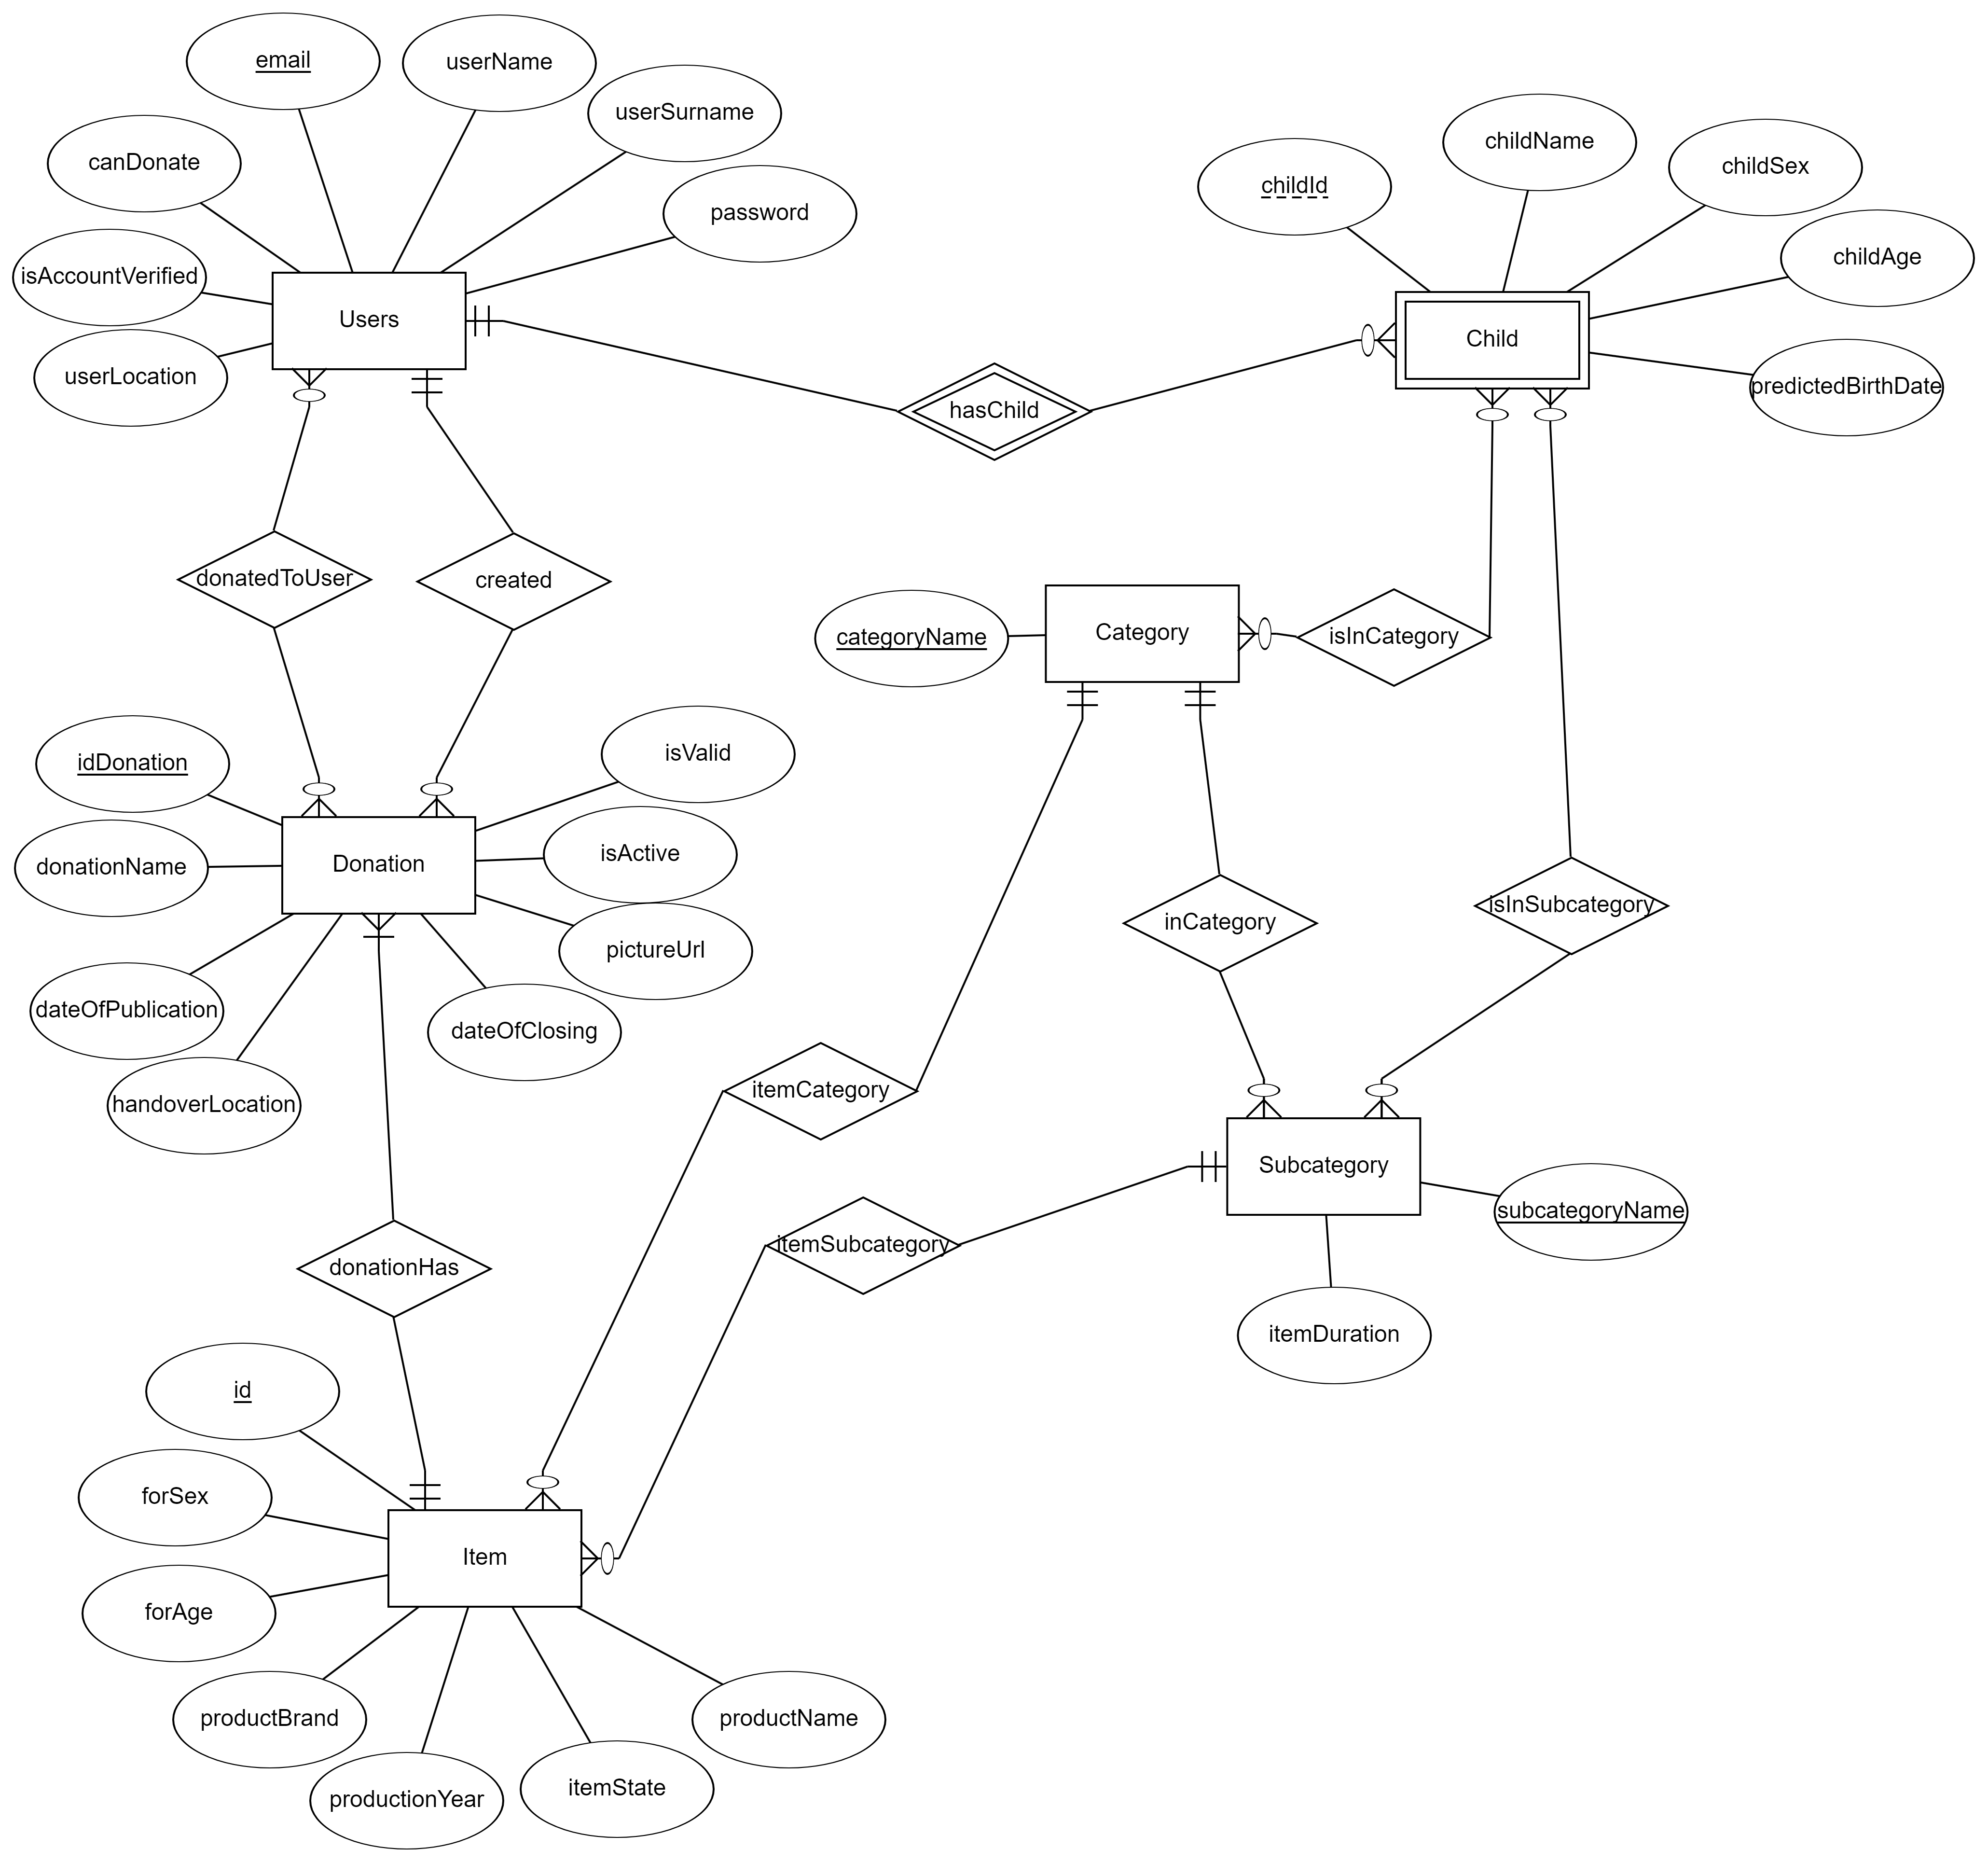
\includegraphics[width=\textwidth,height=0.7\textheight]{dijagrami/ERdijagram.png}
					\centering
					\caption{ER dijagram - aplikacija Djeca za djecu}
					\label{fig:ERDiagram}
				\end{figure}

				\begin{figure}[H]
					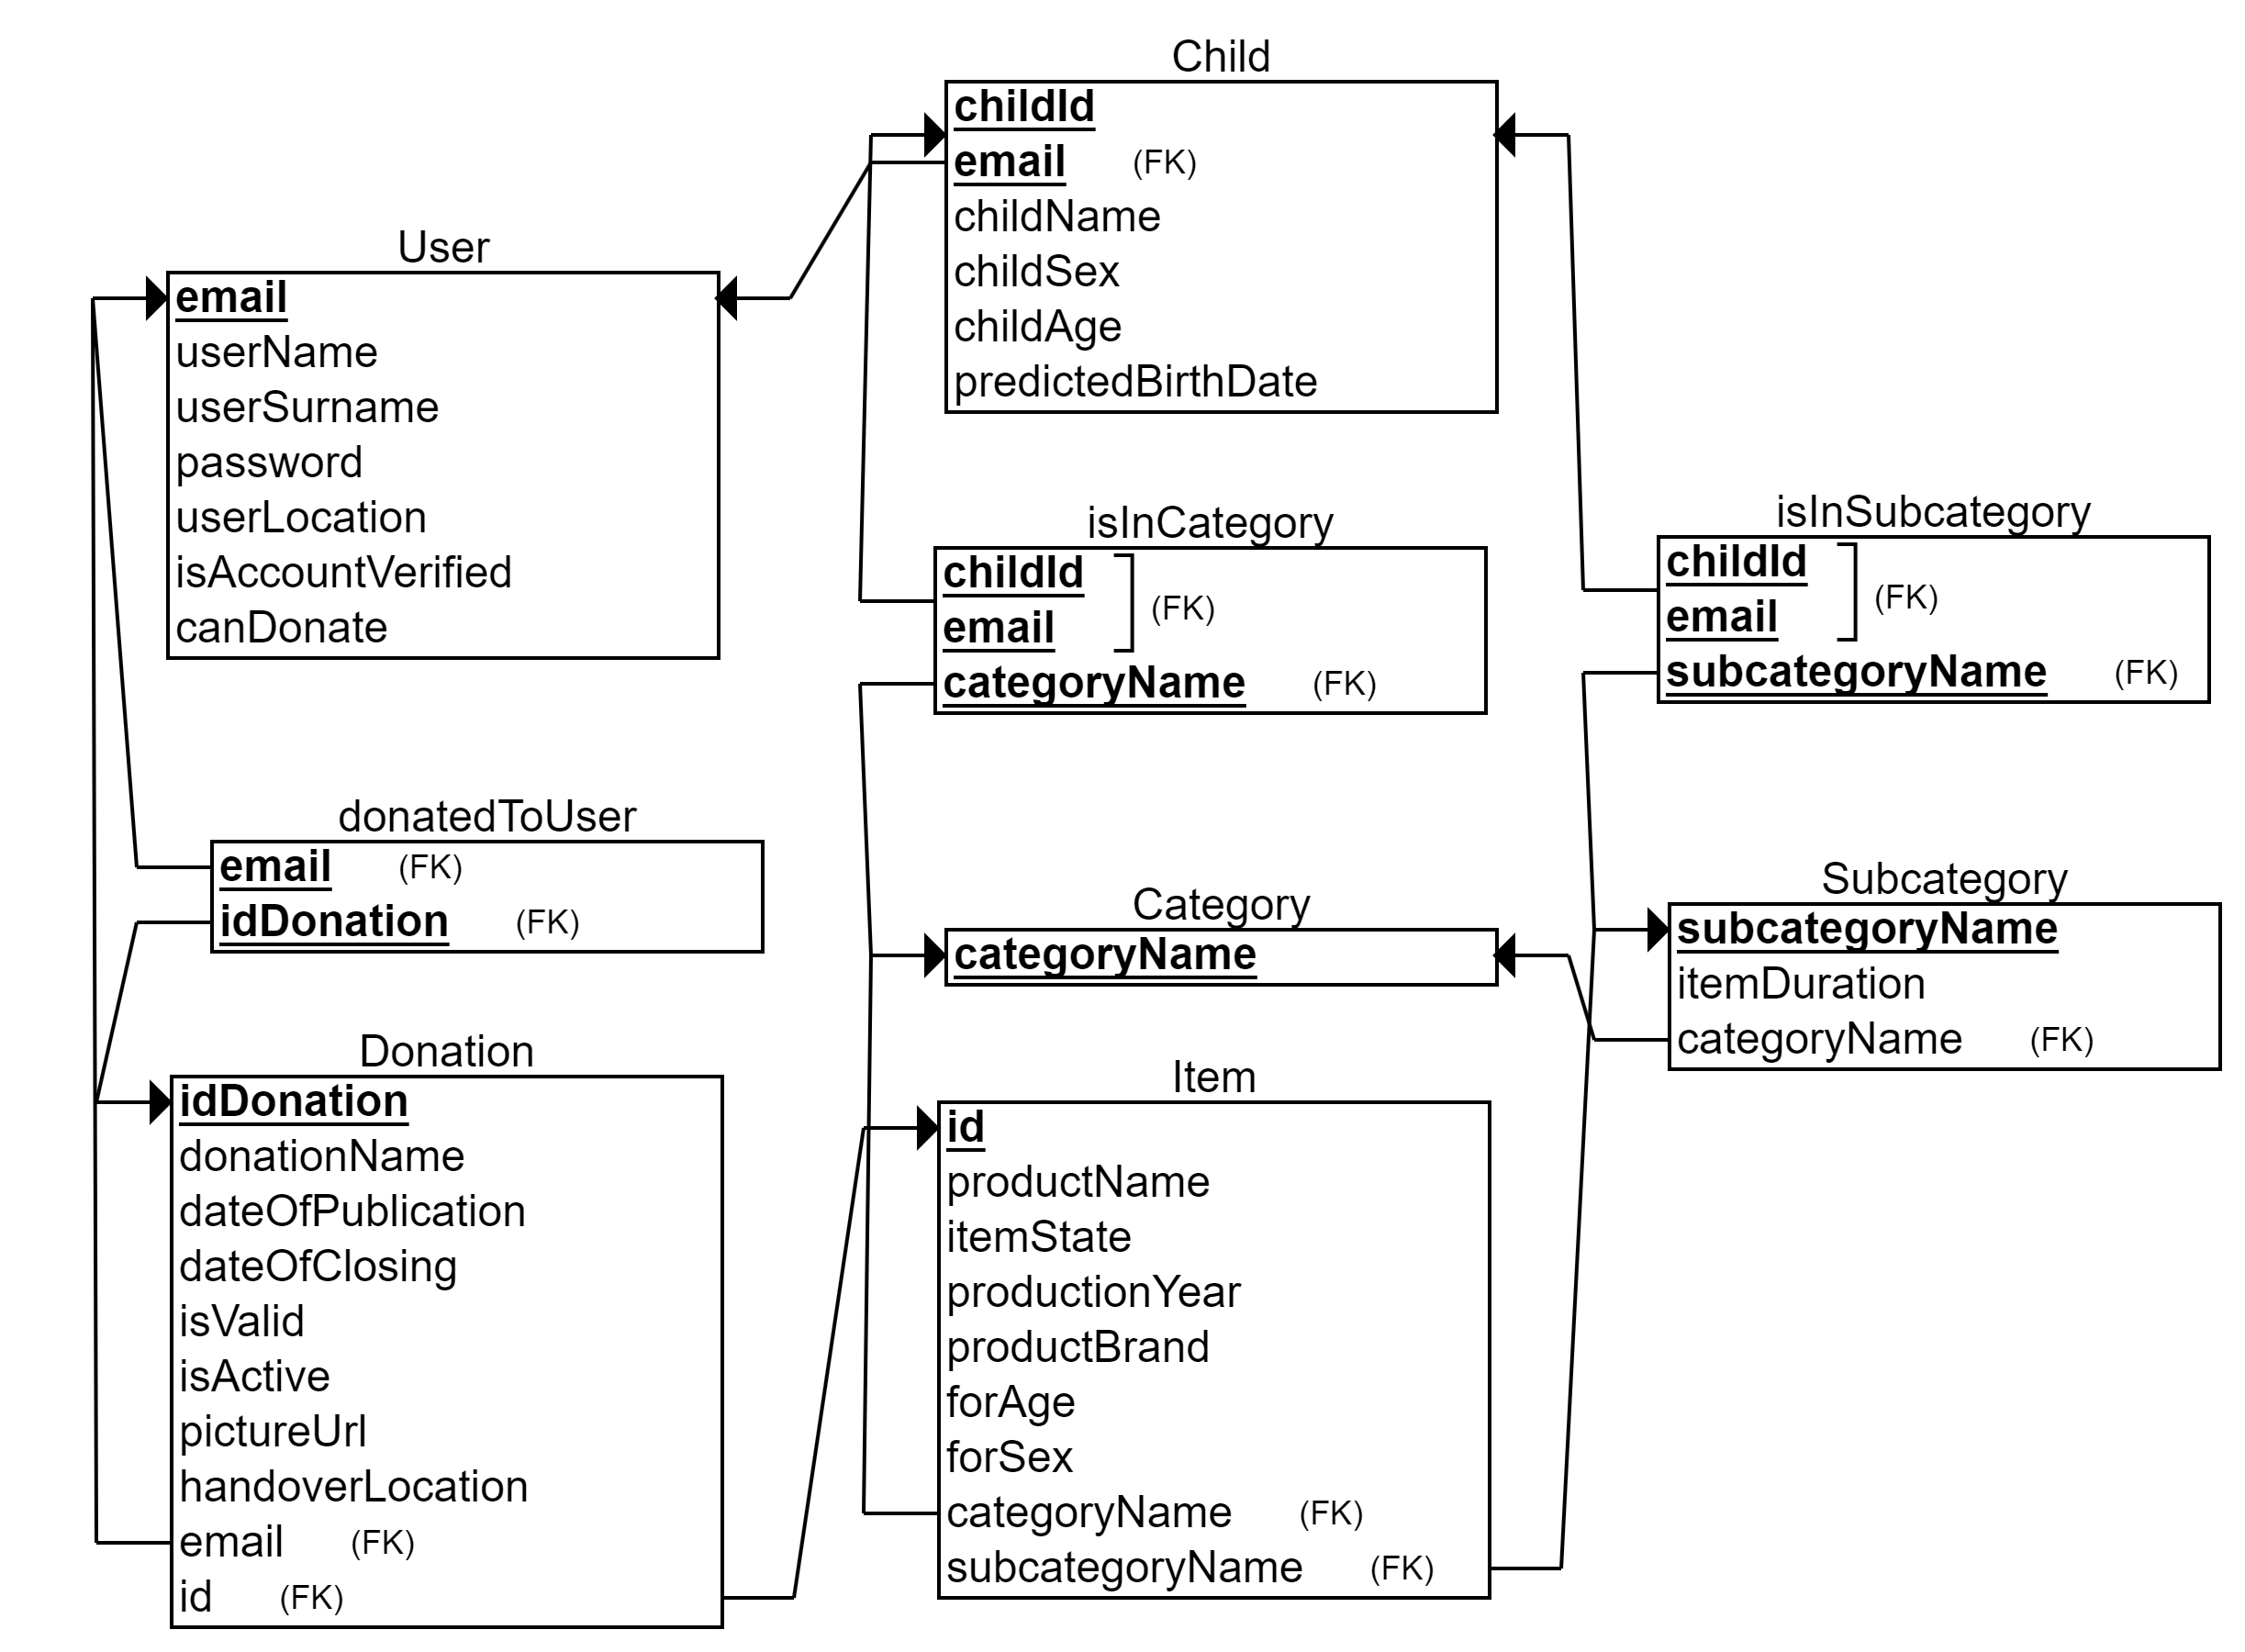
\includegraphics[width=\textwidth,height=0.7\textheight]{dijagrami/RelDijagram.png}
					\centering
					\caption{Relacijski dijagram - aplikacija Djeca za djecu}
					\label{fig:RelDijagram}
				\end{figure}
			\eject
			
			
		\section{Dijagram razreda}
			
			%\textbf{\textit{dio 1. revizije}}\\
			
			%\textit{Prilikom prve predaje projekta, potrebno je priložiti potpuno razrađen dijagram razreda vezan uz \textbf{generičku funkcionalnost} sustava. Ostale funkcionalnosti trebaju biti idejno razrađene u dijagramu sa sljedećim komponentama: nazivi razreda, nazivi metoda i vrste pristupa metodama (npr. javni, zaštićeni), nazivi atributa razreda, veze i odnosi između razreda.}\\
			
			Na slikama 4.4 do 4.7 prikazani su razredi koji pripadaju backend dijelu našeg sustava.\\[5pt]

			Slika 4.4 prikazuje razrede koji predstavljaju modele - preslikane relacije baze podataka. Razred User predstavlja registriranog korisnika sustava. Razred Child predstavlja dijete registriranog korisnika sustava. Razred Donation predstavlja jednu donaciju zabilježenu u sustavu. 
			Razred Item predstavlja jedan predmet vezan za neke od donacija. Razred Category predstavlja podatke o jednoj od kategorija u koje mogu biti svrstani predmeti. Razred Subcategory predstavlja podatke o jednoj od potkategorija u koje mogu biti svrstani predmeti.\\[10pt]

			\begin{figure}[H]
				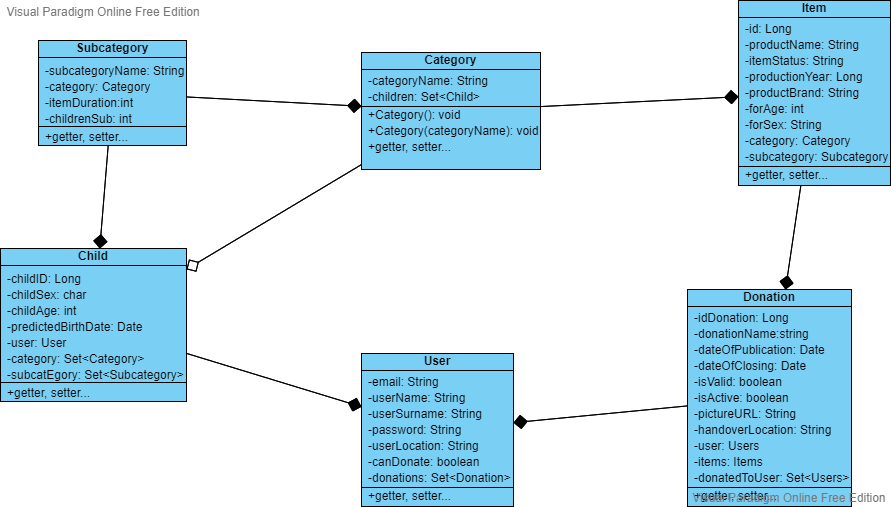
\includegraphics[width=\textwidth,height=0.35\textheight]{dijagrami/Modeli.png}
				\centering
				\caption{Dijagram razreda - dio Models}
				\label{fig:Models}
			\end{figure}
			\eject
			Slika 4.5 prikazuje odnos komponenti na primjeru razreda Category. Razred CategoryController prihvaća i odgovara na HTTP zahtjeve poslane od korisnika tj. konkretnije frontenda. Kako bi na njih ispravno odgovorio, uspostavlja komunikaciju s razredom CategoryServiceJpa.
			Razred CategoryServiceJpa uspostavlja komunikaciju s razredom CategoryService koji obavlja potrebne izračune i provođenje poslovne logike. Isto tako, razred CategoryServiceJpa uspostavlja komunikaciju i s razredom CategoryRepository koji služi kao sučelje za pohranu i dohvat podataka iz baze.
			Kako bi prikaz bio što sažetiji, odnos komponenti prikazan je samo na jednom razredu. U stvarnoj implementaciji, ovakav odnos komponenti tj. razreda postoji za svaki razred iz dijela Models.\\[10pt]

			\begin{figure}[H]
				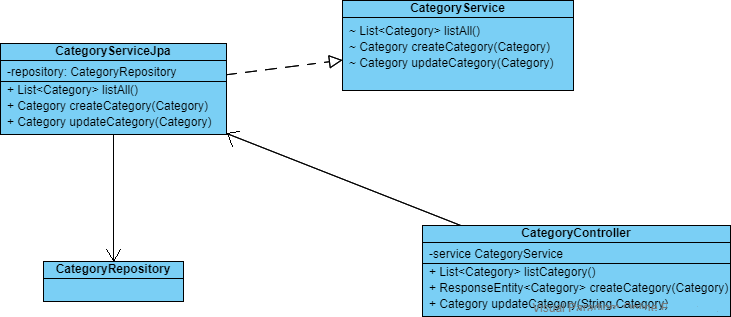
\includegraphics[width=\textwidth,height=0.35\textheight]{dijagrami/OdnosKomponenti.png}
				\centering
				\caption{Dijagram razreda - odnos komponenti}
				\label{fig:OdnosKomponenti}
			\end{figure}

			\eject

			Slika 4.6 prikazuje razrede izvedene iz razreda RestController. Svaki od razreda izvedenih iz RestController služi za prihvaćanje i odgovor na HTTP zahtjeve poslane od strane korisnika tj. konkretnije frontenda.\\[10pt]
			%Razred UsersController služi za slanje odgovora na zahtjeve vezane uz podatke o korisnicima.
			%Razred UsersDetailsService služi za slanje odgovora na zahtjeve vezane uz detaljne podatke o korisnicima.
			%Razred RolesController služi za slanje odgovora na zahtjev vezan uz podatke o ulogama korisnika.
			%Razred ChildController služi za slanje odgovora na zahtjeve vezane uz podatke o djeci.
			%Razred ItemController služi za slanje odgovora na zahtjeve vezane uz podatke o predmetima iz donacija.
			%Razred DonationController služi za slanje odgovora na zahtjeve vezane uz podatke o donacijama.
			%Razred CategoryController služi za slanje odgovora na zahtjeve vezane uz podatke o kategorijama.
			%Razred SubcategoryController služi za slanje odgovora na zahtjeve vezane uz podatke o potkategorijama.\\[10pt]

			\begin{figure}[H]
				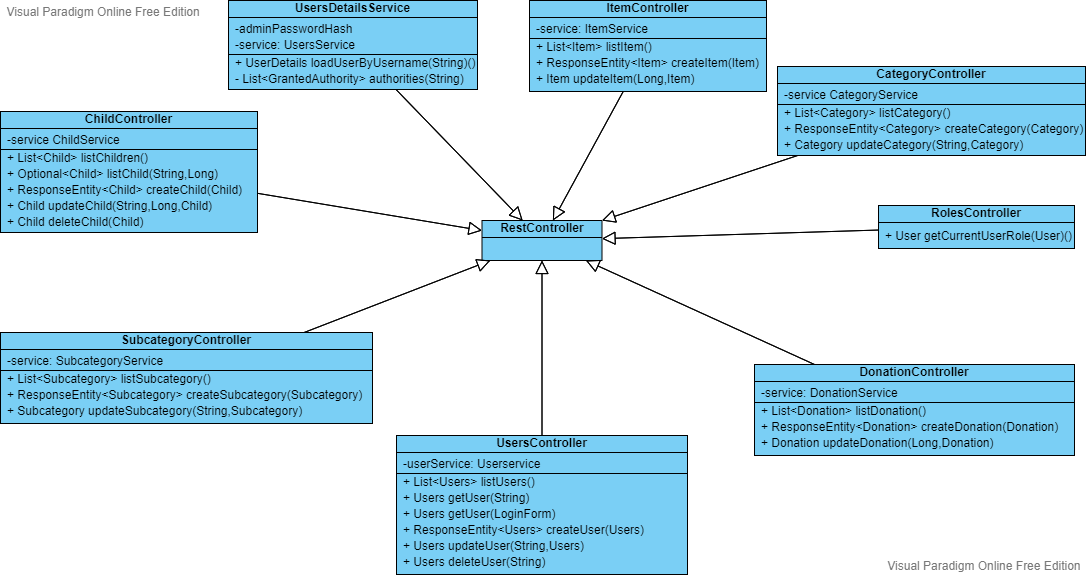
\includegraphics[width=\textwidth,height=0.4\textheight]{dijagrami/Controlleri.png}
				\centering
				\caption{Dijagram razreda - dio Controllers}
				\label{fig:Controllers}
			\end{figure}

			\eject

			Slika 4.7 prikazuje razrede izvedene iz razreda JpaRepository. Svaki od prikazanih razreda služi kao sučelje za pohranu i dohvat podataka iz baze podataka za svoju pripadajuću relaciju.\\[10pt]

			\begin{figure}[H]
				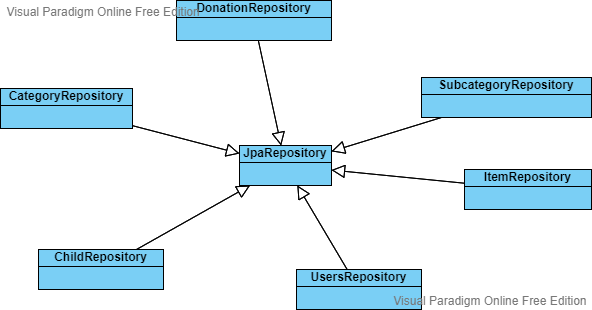
\includegraphics[width=\textwidth,height=0.4\textheight]{dijagrami/Repozitoriji.png}
				\centering
				\caption{Dijagram razreda - dio Repositories}
				\label{fig:Repositories}
			\end{figure}

			%\textbf{\textit{dio 2. revizije}}\\			
			
			%\textit{Prilikom druge predaje projekta dijagram razreda i opisi moraju odgovarati stvarnom stanju implementacije}
			
			
			
			\eject
		
		%\section{Dijagram stanja}
			
			
			%\textbf{\textit{dio 2. revizije}}\\
			
			%\textit{Potrebno je priložiti dijagram stanja i opisati ga. Dovoljan je jedan dijagram stanja koji prikazuje \textbf{značajan dio funkcionalnosti} sustava. Na primjer, stanja korisničkog sučelja i tijek korištenja neke ključne funkcionalnosti jesu značajan dio sustava, a registracija i prijava nisu. }
			
			
			%\eject 
		
		%\section{Dijagram aktivnosti}
			
			%\textbf{\textit{dio 2. revizije}}\\
			
			 %\textit{Potrebno je priložiti dijagram aktivnosti s pripadajućim opisom. Dijagram aktivnosti treba prikazivati značajan dio sustava.}
			
			%\eject
		%\section{Dijagram komponenti}
		
			%\textbf{\textit{dio 2. revizije}}\\
		
			% \textit{Potrebno je priložiti dijagram komponenti s pripadajućim opisom. Dijagram komponenti treba prikazivati strukturu cijele aplikacije.}